%%%%%%%%%%%%%%%%%%%%%%%%%%%%%%%%%%%%%%%%%%%%%%%%%%%%%%%%%%%%%%%%%%%
%                                                                 %                    
%                 Packages / Grundeinstellungen                   %
%                                                                 %
%%%%%%%%%%%%%%%%%%%%%%%%%%%%%%%%%%%%%%%%%%%%%%%%%%%%%%%%%%%%%%%%%%%
\DocumentMetadata{
    pdfversion=2.0,
    pdfstandard=A-4,
}

\documentclass[paper=a1,parskip=half,fontsize=24]{scrartcl}

\usepackage[ngerman]{babel}
\usepackage{lmodern}
\usepackage{fontspec}
\usepackage{calc}
\usepackage{microtype}
\usepackage{tcolorbox}
\usepackage{blindtext}
\usepackage{float}
\usepackage{subcaption}

% Keine floats in andere Sections
\usepackage[section]{placeins}

% Eurozeichen einbinden
\usepackage[right]{eurosym}

% Floatende Bilder ermöglichen
\usepackage{floatflt}

% Bricht lange URLs "schön" um
\usepackage[hyphens,obeyspaces,spaces]{url}

% Mathematische Symbole importieren
\usepackage{amssymb}

% Zitierung nach APA
%\usepackage[
%backend=biber,
%style=apa,
%autocite=inline,
%]{biblatex}
%\addbibresource{bibtex/poster.bib}

% Zitierung nach IEEE
\usepackage[
backend=biber,
style=ieee,
autocite=inline,
]{biblatex}
\addbibresource{bibtex/poster.bib}

\setcounter{biburllcpenalty}{7000}
\setcounter{biburlucpenalty}{8000}

% Paket für Zeilenabstand
\usepackage{setspace}

% Für Bildbezeichner
\usepackage{capt-of}

% Für Stichwortverzeichnis
\usepackage{makeidx}

% Erzeugt Inhaltsverzeichnis mit Querverweisen zu den Abschnitten (PDF Version)
\usepackage[bookmarksnumbered,hyperfootnotes=false,hypertexnames=false]{hyperref}
\hypersetup{
  colorlinks=true,
  linkcolor=black,
  filecolor=blue,
  citecolor = black,      
  urlcolor=blue,
  }

%mehrspaltig
\usepackage{multicol} 
\columnsep=70pt 
\columnseprule=3pt 

%grafiken einbinden
\usepackage{graphicx}

% Booktabs Tabellen
\usepackage{tabularray}
\UseTblrLibrary{booktabs}
\DefTblrTemplate{contfoot-text}{normal}{Fortsetzung auf nächster Seite}
\SetTblrTemplate{contfoot-text}{normal}
\DefTblrTemplate{conthead-text}{normal}{}
\SetTblrTemplate{conthead-text}{normal}

% Paket für Textfarben
\usepackage{xcolor} 
\definecolor{LightGray}{gray}{0.9}
\usepackage[pagecolor=white]{pagecolor}

% Für schönere Listings
\usepackage[outputdir=log, newfloat,]{minted}
\setminted{
  frame=lines,
  framesep=2mm,
  baselinestretch=1.2,
  bgcolor=LightGray,
  fontsize=\footnotesize,
  linenos,
  breaklines=true,
  breakanywhere=true,
  autogobble,
  tabsize=2
}
\setmintedinline{}

% Keine Floats bei Listings
\newenvironment{code}[2]
  {
  \providecommand{\captiontitle}{#1}
  \providecommand{\labeltitle}{#2}
  \vspace*{0.3cm}
  }
  {
  %\vspace*{-2.0cm}
  \captionbelowof{listing}{\captiontitle}
  \label{\labeltitle}
  \vspace*{0.35cm}
  }
\SetupFloatingEnvironment{listing}{}

%seitengeometrie
\usepackage{geometry}
\geometry{margin=3cm,top=3cm}

%Definition Schrift- und Farbeinstellungen 
\setmainfont{TeX Gyre Termes}
\setsansfont{TeX Gyre Adventor}
\usepackage{preamble}


%Siehe hierzu preamble.sty
\colorlet{basecolor}{meerblau}
\colorlet{akzentcolor}{mint}

%Siehe hierzu preamble.sty
\renewcommand{\theauthor}{Thore Hüneke thohueneke, Anette Michlik anemichlik, Kasem Rashrash kasrashrash, Sophie Sergeenko sopsergeenko}
\renewcommand{\thetitle}{Impftermine digital: Schnell. Sicher. Skalierbar.}
\renewcommand{\thesubtitle}{Das SWE3-Projekt von Team swe3-2024-03}

%Höhe des HS Logos 4cm für zweizeiligen Titel, 2.5cm für einzeiligen Titel
\newcommand{\myspace}{4cm}

\hypersetup{pdfinfo={
  Title={\thetitle},
  Author={\theauthor}
}}

% Darf erst hier eingebunden werden! 
\usepackage{csquotes}

%Textfarbe
\color{black}

%%%%%%%%%%%%%%%%%%%%%%%%%%%%%%%%%%%%%%%%%%%%%%%%%%%%%%%%%%%%%%%%%%%
%                                                                 %                    
%                     Beginn des Inhalts                          %
%                                                                 %
%%%%%%%%%%%%%%%%%%%%%%%%%%%%%%%%%%%%%%%%%%%%%%%%%%%%%%%%%%%%%%%%%%%

%%%%%%%%%%%%%%%%%%%%%%%%%%%%%%%%%%%%%%%%%%%%%%%%%%%%%%%%%%%%%%%%%%%
%  Special Characters:                                            %
%                                                                 %
%             \& \% \$ \# \_ \{ \}                                %
%             \textasciitilde (~)                                 %
%             \textasciicircum (^)                                %     
%             \textbackslash (\)                                  %                    
%      \glqq Text\grqq{} für Anführungszeichen                    %
%%%%%%%%%%%%%%%%%%%%%%%%%%%%%%%%%%%%%%%%%%%%%%%%%%%%%%%%%%%%%%%%%%%


\begin{document}
  %Printed Überschriften
  \thetitlearea
  %Mehrspaltig
  \begin{multicols*}{3}
  
    % Input Inhalt
    \section*{Problemstellung}
Die Stadt Nemreb möchte sich auf künftige Pandemiesituationen besser vorbereiten und ein 
robustes, skalierbares System zur Impfterminregistrierung entwickeln. Ziel ist es, eine 
Webanwendung bereitzustellen, die auch bei hoher Nachfrage stabil und effizient bleibt. 
Die technische Umsetzung stellt verschiedene Herausforderungen, darunter die 
Benutzerverwaltung mit Registrierung und Anmeldung per E-Mail sowie die Terminbuchung, 
bei der Nutzer freie Termine einsehen, buchen und absagen können. Dabei müssen die 
Kapazitäten der Impfzentren berücksichtigt werden, sodass Zeitslots nicht überbucht werden.
Erweiterte Buchungsfunktionen sollen es ermöglichen, Termine auch für Familienmitglieder 
zu reservieren. Zudem wird für jede Buchung ein QR-Code generiert, der in einem 
Bestätigungspdf enthalten ist, wobei der Datenschutz gewahrt bleibt und keine 
persönlichen Daten im QR-Code gespeichert werden. Datenschutz und Sicherheit sind 
zentrale Aspekte des Systems, weshalb auf Transparenz, minimale Datenspeicherung und das 
Hosting in der behördlichen Infrastruktur Wert gelegt wird. Ein weiteres essenzielles 
Kriterium ist die Fehlertoleranz und Skalierbarkeit des Systems, um auch unter hoher Last 
performant zu bleiben und kurzfristige Anpassungen zu ermöglichen.
Zur Optimierung der Systemstabilität wird ein Echtzeit-Monitoring der Systemauslastung 
integriert, sodass auf Engpässe schnell reagiert werden kann. Das System soll als 
Open-Source-Projekt entwickelt werden und auf einem aktuellen Tomcat-Server mit einer 
Open-Source-Datenbank unter Linux betrieben werden. Durch die Verwendung eines 
reduzierten Technologie-Stacks wird eine langfristige Wartbarkeit gewährleistet, während 
bewusst auf komplexe Frameworks verzichtet wird, um Transparenz zu erhöhen. Solide Tests 
und Continuous Integration werden eingesetzt, um die Softwarequalität sicherzustellen und 
die Zusammenarbeit zwischen Unix-Administratoren und Java-Entwicklern zu verbessern.
Durch dieses Konzept wird eine effiziente und skalierbare Impfregistrierung 
gewährleistet, die Ausfälle vermeidet und eine hohe Benutzerakzeptanz sichert. Die 
schnelle Reaktionsfähigkeit auf Systemänderungen und Lastspitzen stellt eine weitere 
Stärke dar. Zudem bietet das System eine nachhaltige und wiederverwendbare Lösung, die 
auch in anderen Kommunen Anwendung finden kann. Damit wird eine zuverlässige technische 
Grundlage für künftige Impfkampagnen geschaffen.

    \section*{Nutzer}
Wer nutzt das system?

\begin{center}
  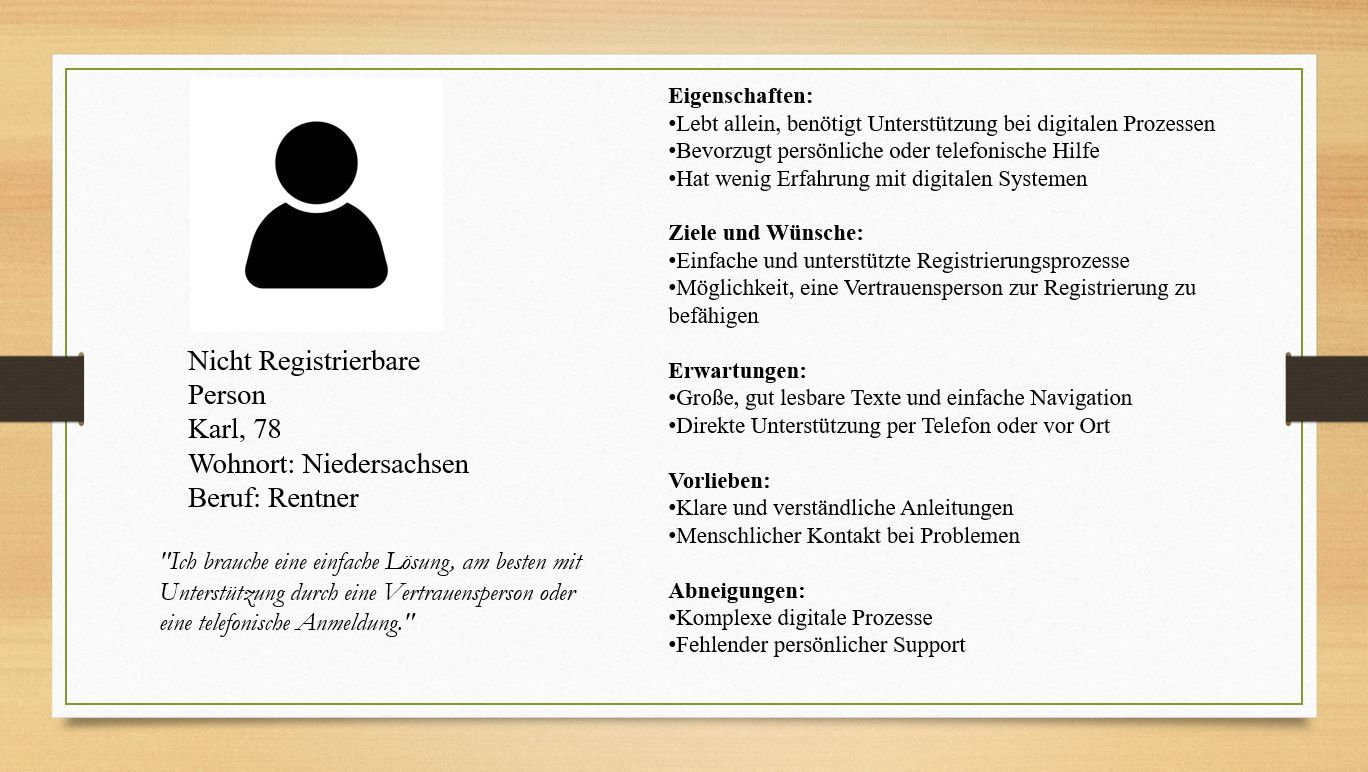
\includegraphics[width=0.95\linewidth, height=0.45\textheight, keepaspectratio]{src/abbildungen/persona1.png}
  \captionof{figure}{Persona 1}
\end{center}

\begin{center}
  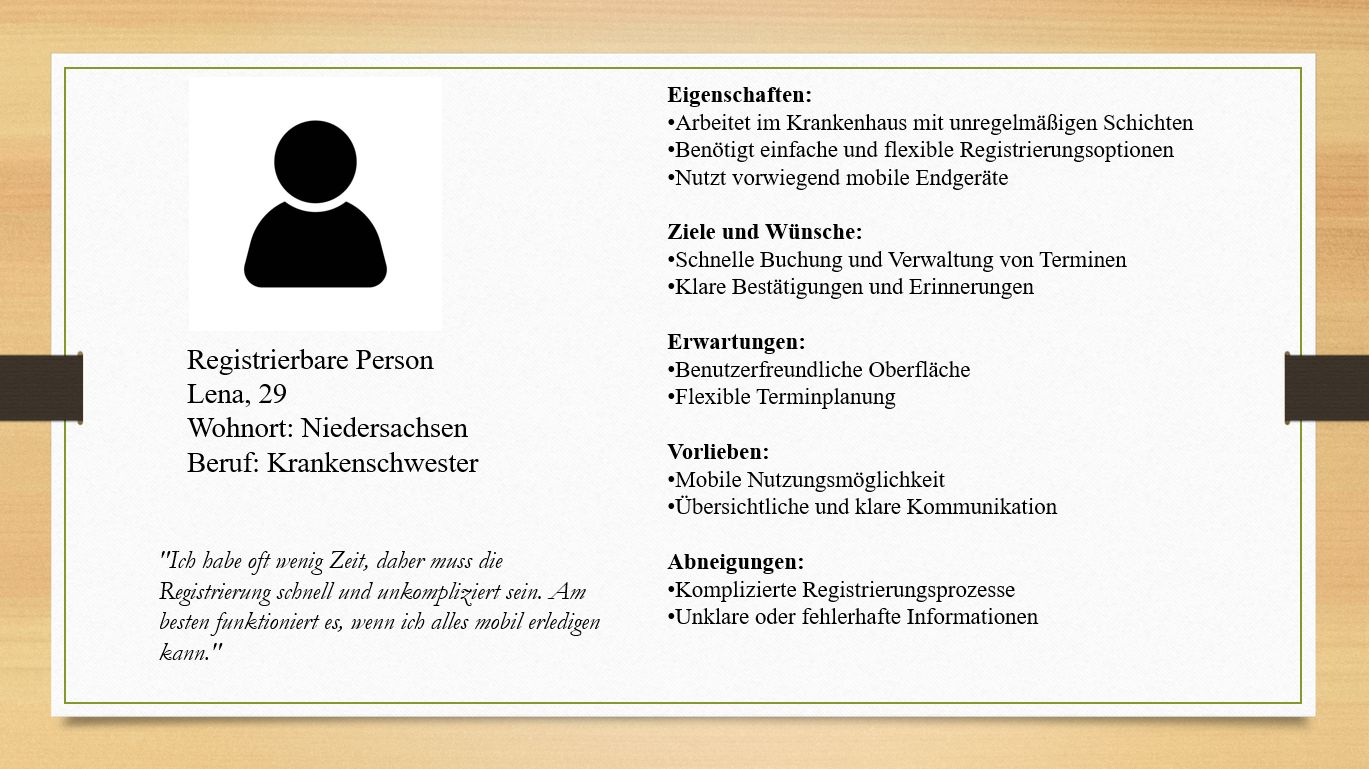
\includegraphics[width=0.95\linewidth, height=0.45\textheight, keepaspectratio]{src/abbildungen/persona2.png}
  \captionof{figure}{Persona 2}
\end{center}


%\begin{figure}[H]
%  \centering
%  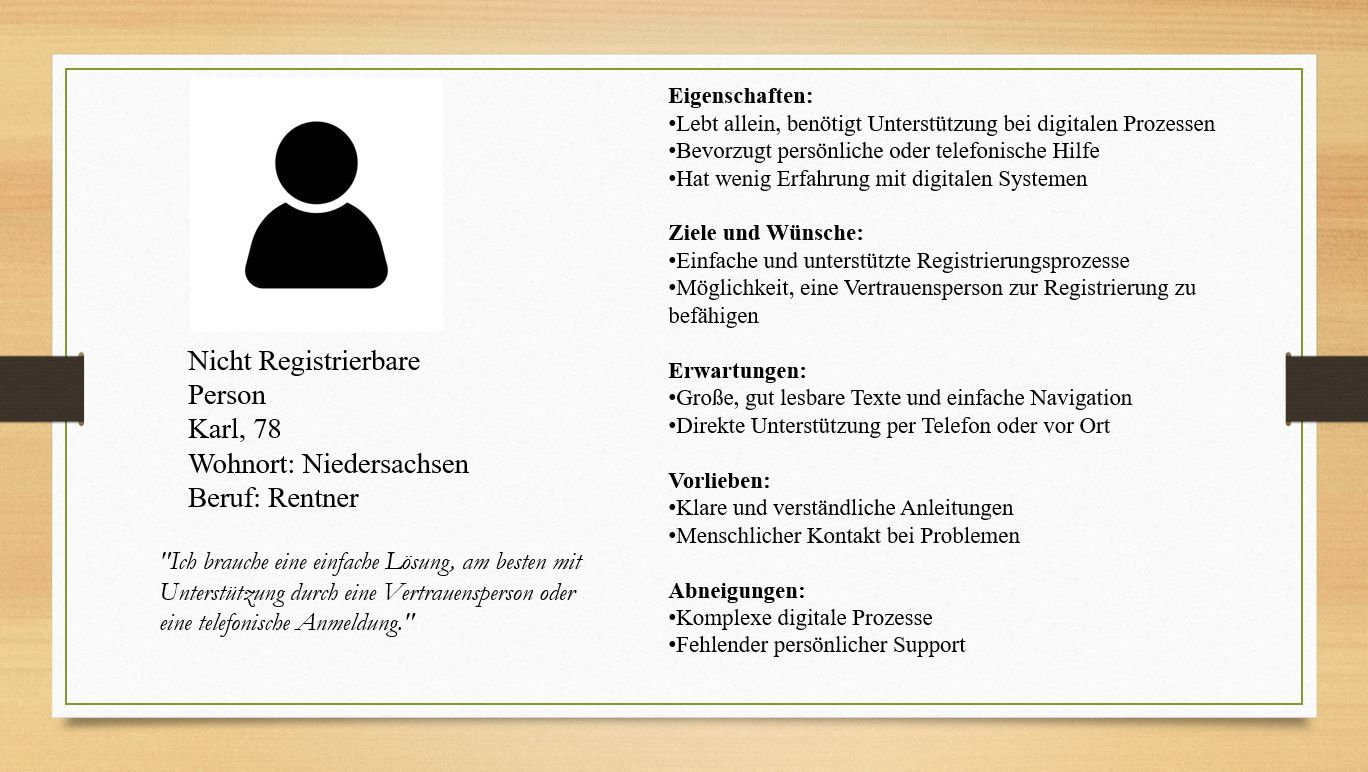
\includegraphics[scale=0.3]{src/abbildungen/persona1.png}
%  \caption{Persona 1}
%\end{figure}

%\begin{figure}[H]
%  \centering
%  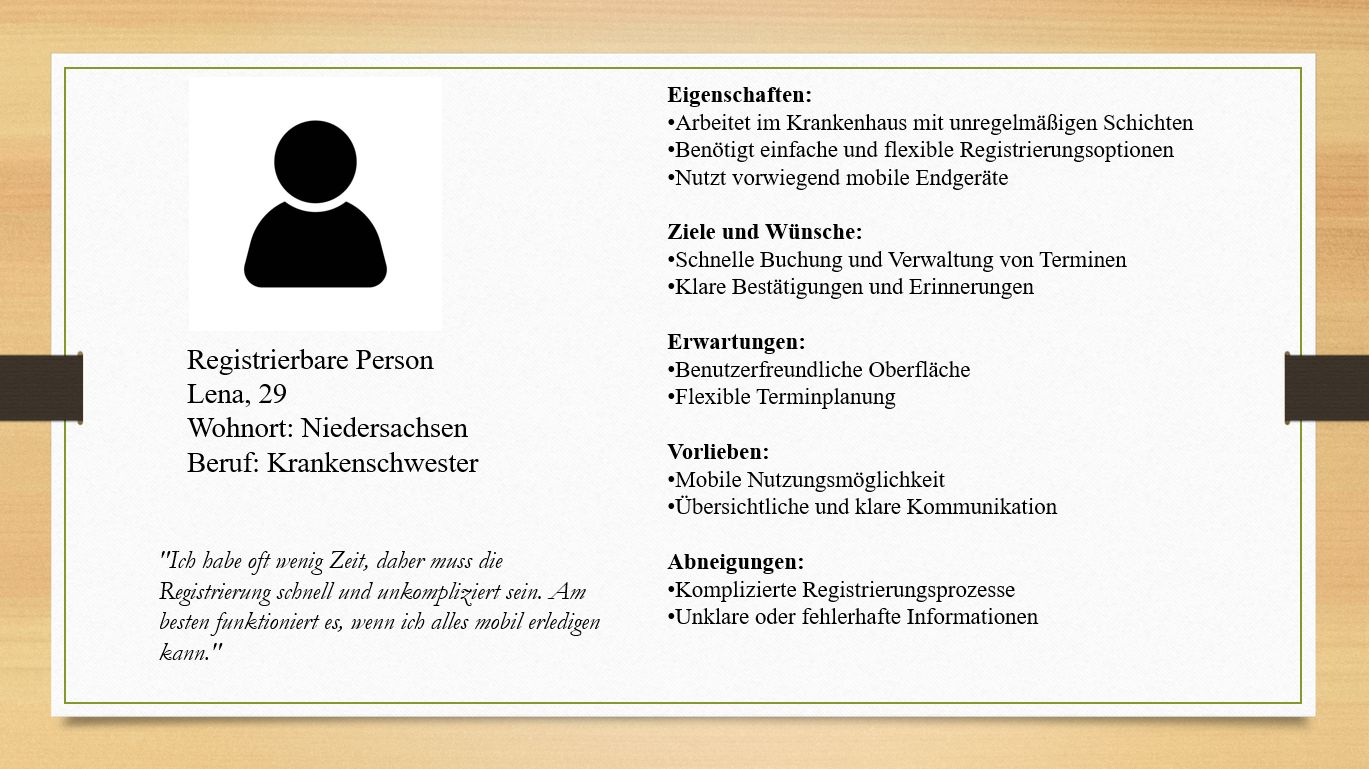
\includegraphics[scale=0.3]{src/abbildungen/persona2.png}
%  \caption{Persona 2}
%\end{figure}

    \section*{Anforderungen}


\subsection{Funktionale Anforderungen}

WAS MUSS DAS SYSTEM KÖNNEN?

Benutzerregistrierung & Anmeldung
Terminbuchunug & stornierung
qr-code generierung 
?????

\subsection{Nicht-Funktionale Anforderungen}

WIE SOLL DAS SYSTEM ARBEITEN

hohe verfügbarkeit & skalierbarkeit
datenschutz und sicherheit
open source

????

    \section*{Ablauf}

Wie funktioniert die Terminbuchung ? 

Nutzer meldet sich an
verfpgabre termine werden angezeigt
bucht termin
erhält bestätigung mit qr code
qr code wird im impfzentrum gescannt?????

use-case && aktivitätsdiagramme als BILD

\begin{center}
 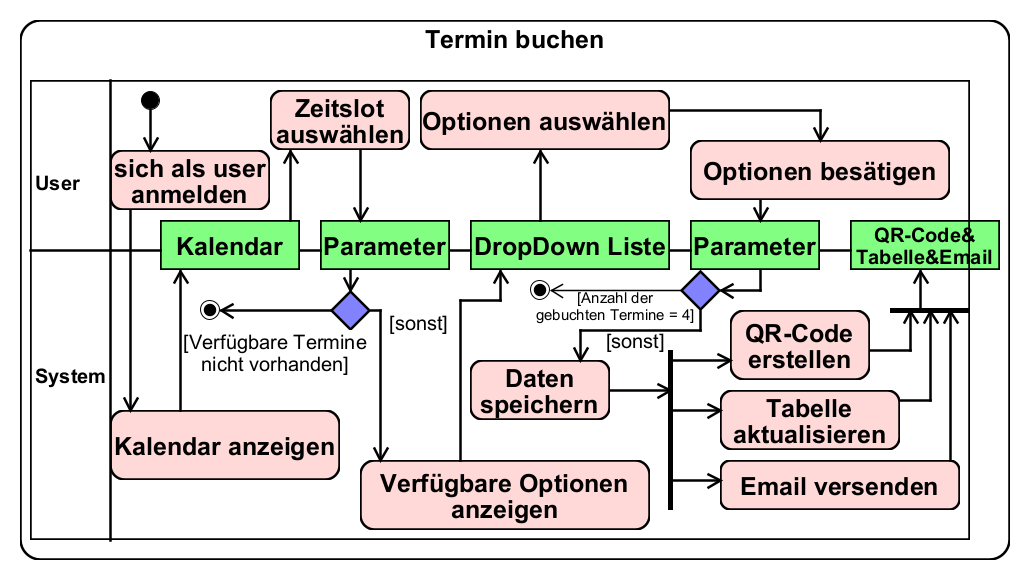
\includegraphics[width=0.35\textwidth, height=1.45\textheight, keepaspectratio]{src/abbildungen/activity.png}
  \captionof{figure}{Persona 1}
\end{center}

\begin{center}
  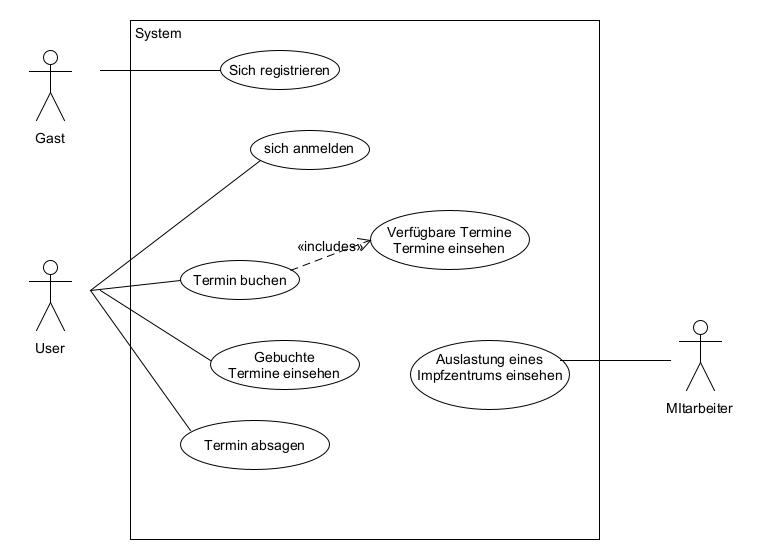
\includegraphics[width=0.95\linewidth, height=0.45\textheight, keepaspectratio]{src/abbildungen/usecases.jpg}
  \captionof{figure}{Persona 2}
\end{center}


%%\begin{figure}[H]
%  \centering
%  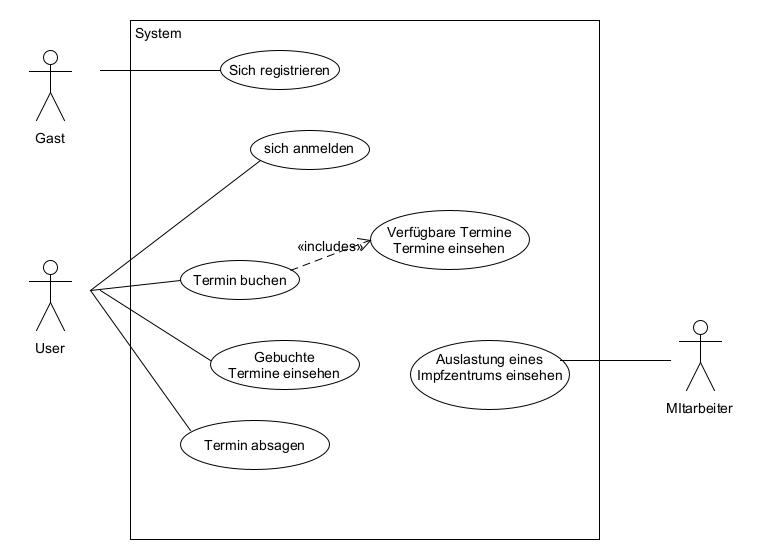
\includegraphics[scale=0.3]{src/abbildungen/usecases.jpg}
%  \caption{Usecases}
%\end{figure}

%\begin{figure}[H]
%  \centering
%  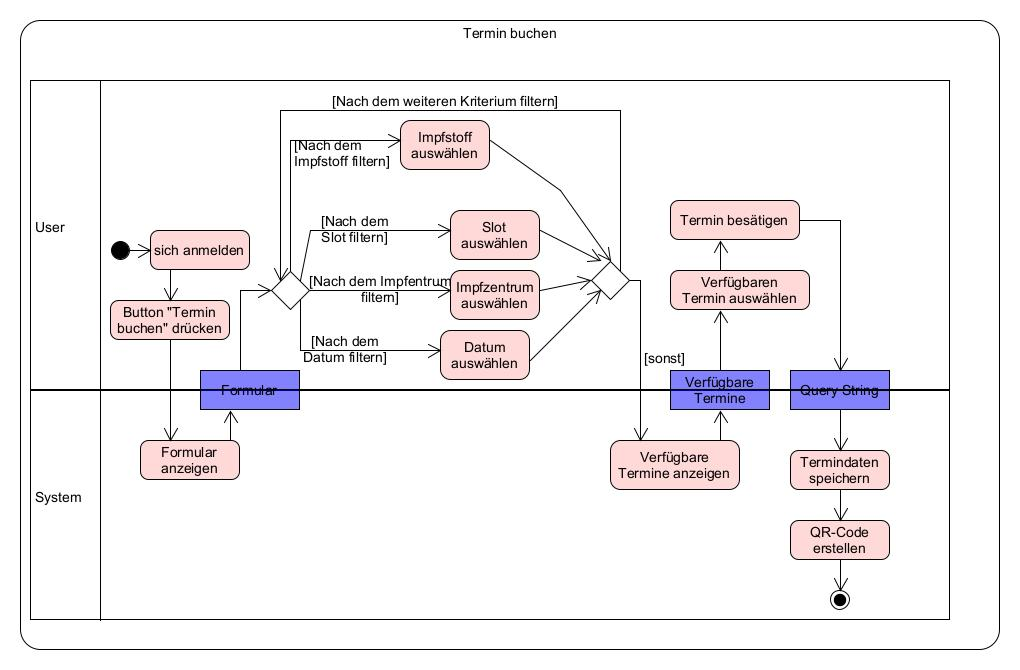
\includegraphics[scale=0.3]{src/abbildungen/terminbuchen.jpg}
%  \caption{Aktivität Termin buchen}
%\end{figure}

    \section*{Design}

wie sieht das system aus ? 

bilder rein 

für alle rollen
nutzer und mitarbeiter

    
    % Literaturverzeichnis anzeigen
    %\section*{Referenzen}
    %\vspace*{0.3cm}
    %\printbibliography[heading=none]

  \end{multicols*}
\end{document}

